\documentclass[signature=data]{physicsreport}

%%
%% User settings
%%

\classno{}
\stuno{}
\groupno{}
\stuname{}
\expdate{\expdatefmt\today}
\expname{迈克尔逊干涉仪实验}

%%
%% Document body
%%

\begin{document}
% First page
% Some titles and personal information are defined in ``\maketitle''.
\maketitle

\section{预习}
\begin{enumerate}
    \item 结合下图迈克尔逊干涉仪的等效光路图,推导出光程差的表达式$\Delta L = 2hcos\alpha$。
    \begin{figure}[htbp]
    \flushright
    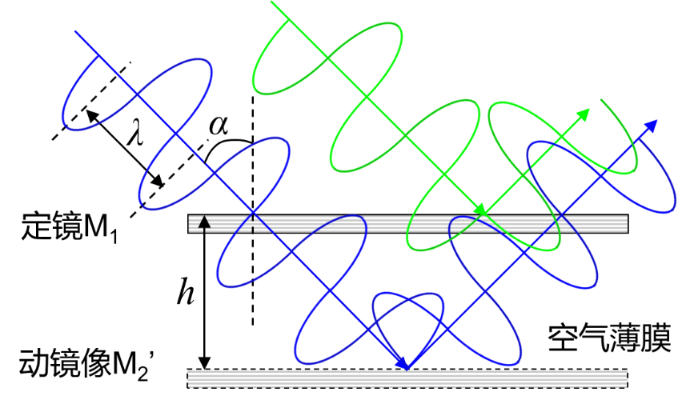
\includegraphics{images/figure1.png}
    \end{figure} 
    \vspace{3cm}
    \item 本实验将测量He-Ne激光的波长$\lambda$,若等倾干涉圆环每变化50环,动镜$M_2$对应的螺旋测微器读数变化为$d$(注意:$M_2$实际移动距离为$d/20$),根据光程差的表达式光程差$\Delta L = 2hcos\alpha$,结合中心圆环对应的倾角$\alpha \approx 0$这一近似条件,推导出波长$\lambda$的表达式(提示:光程差每改变1个波长,干涉圆环变化1环)。
    \vspace{5cm}
\end{enumerate}

% Teacher signature
\makeatletter
\physicsreport@body@signature{preparation}
\makeatother

\section{实验目的及任务}
\begin{enumerate}
    \item 了解迈克尔孙干涉仪的结构、原理及调节方法;
    \item 观察光的非定域和定域干涉现象,包括等倾和等厚干涉;
    \item 逐差法测定He-Ne激光波长;
    \item 作图法计算空气的折射率。
\end{enumerate}
\vspace{0.7cm}
% Original experiment data
\section{原始数据记录}
\subsection{}
\begin{table}[H]
    \caption{测定 He-Ne 激光波长数据} \label{tab:1}
    \centering
    \begin{tabularx}{\textwidth}{|c|Y|Y|Y|Y|Y|Y|} \hline
        圆环变化数目          & 0 & 50 & 100 & 150 & 200 & 250 \\\hline
        $M_2$ 位置读数 (mm) &   &    &     &     &     &     \\\hline
    \end{tabularx}
\end{table}

\subsection{}
\begin{table}[H]
    \caption{测定空气折射率数据} \label{tab:2}
    \centering
    \begin{tabularx}{\textwidth}{|c|Y|Y|Y|Y|Y|} \hline
        气室内压强 (mmHg) & 50 & 100 & 150 & 200 & 250 \\\hline
        干涉条纹变化数      &    &     &     &     &     \\\hline
        干涉条纹变化数      &    &     &     &     &     \\\hline
        干涉条纹变化数      &    &     &     &     &     \\\hline
    \end{tabularx}
\end{table}

\subsection{观察等倾和等厚现象, 并附现象图.}

% Teacher signature
\makeatletter
\physicsreport@body@signature{data}
\makeatother

\newpage
% Data process and others
\section{数据处理}
\begin{enumerate}
    \item 利用逐差法计算 He-Ne 激光波长.
    \vspace{3cm}
    \item 作出条纹变化数 $\Delta n$ 相对于气压变化 $\Delta p$ 的曲线, 用图解法计算斜率, 求出空气的折射率.
    \vspace{3cm}
    \item 记录等倾和等厚现象, 特点并分析.
    \vspace{3cm}
\end{enumerate}


\section{讨论题}
\begin{enumerate}
    \item 归纳非定域干涉和定域干涉的特点.
    \vspace{3cm}
    \item 迈克尔逊干涉仪所产生的干涉条纹疏密程度是由什么因素决定的? 变化规律怎样?
    \vspace{3cm}
    \item 说明仪器要设计补偿片的原因.
\end{enumerate}

\end{document}
